\chapter{Work Plan}

The main goal of this work is to add new functionalities in the current HEP-Frame version, namely to integrate support in this framework for specification and execution of conditional task graphs. This allows HEP-Frame to support a wider range of pipelined applications, while employing the existing optimization strategies for conventional task graphs, as well as implement new scheduling strategies for task pipelines that require conditional paths of execution.
Most task schedulers use conventional execution graphs, where  the nodes represent tasks and the directed connections among them represent possible execution flows between tasks [1-9]. Conditional task graphs may not be possible to express as a traditional execution graph, as a single graph representation must include (i) dependencies among tasks, (ii) conditional paths of execution, and (iii) the filtering out of elements, preventing them from being executed by the remaining tasks. An adequate graph representation must be designed, as it is key to develop efficient strategies to schedule these tasks among workers.

\section{Proposed approach}
%\subsection{Ja detalhes concretos de como se deveria estruturar e implementar as coisas}



The developed scheduler should be accompanied by other tools to automatically parse a predefined signature of a task and identify its dependencies, identify data dependencies, validate the created graph, and measure several metrics useful for the scheduler. These tools should be efficient in order to either operate at compile- or run-time, depending on their purpose. Once validated in a contained code base, the scheduler and these tools should be integrated into HEP-Frame.
This way we can structure our project in the following components:
\begin{itemize}
    \item Preprocessor
    \item Graph Creator
    \item Graph validator
    \item Conditional Validator
    \item Scheduler
\end{itemize}

\begin{figure}[h]
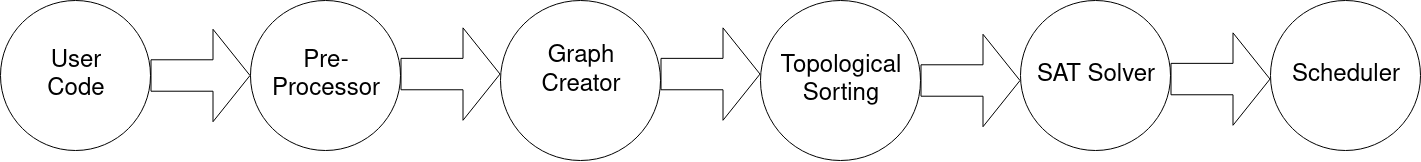
\includegraphics[width=15cm]{img/Tools-pipeline}
\end{figure}

This way the preprocessor, graph creator and graph validation run before compilation with a pipeline like behaviour.
This process will  occur before compilation and its end result will end up being an header file with an enum that attributes an integer to each of the user defined functions and a separated file with the graph definition to be used in the scheduler.


%\subsection{Definicao do prototipo das tarefas (restricoes e codigo}

%****como se definiu a sintaxe (ex, porque nao usar vars globais)
%****explicar o mecanismo de CRIAR e PASSAR de Prop2 para um valor qe o escalonador entenda

This scheduler will execute the functions defined by the user that have the following interface 
\begin{lstlisting}
#include "props.h"

int prop1(int id, Data data) { 
    if(...) 
        return Prop2; 
    if(...) 
        return Prop3; 
    if(...) 
        return FAIL; 
}
\end{lstlisting}
with this interface we can pass a thread id for the scheduler and the data field for the dataset that is being executed right now. Together with the header file we can distinguish the user defined functions from the rest of the code.
With all the pre processor steps finished and all the validations a prop header file is created to allows us to define a Enum interface for all the defined function so to get a final function equivalent to this:

\begin{lstlisting}
int Prop1(....) { 
    if(...) 
        return 1; 
    if(...) 
        return 2; 
    if(...) 
        return -1; 
} 
\end{lstlisting}{}
that will be able to actually able to compile.




%\subsection{qual o pre processamento e como o fazer concretamente (tudo desde criar Dag, se as dependencias sao validas,etc}
The preprocessor will be a separate program that parses the source files written by the user and by the context given witha the function definitons and the imported source files we can uderstand what are the functions belonging to our pipeline. After parsing this functions we create a file that describes the inter connections of all the tasks, wich will form a graph.
After this the file will pass a validation process, wich will detect any possible cycle with topological sorting, (Also Known as Dependency resolution) if we want to have acyclic graph and need to order the tasks that constitute them then this seems the best option, because it can check both properties at the same time.
With the graph validated we then need to validate the condition that decide if a certain branch of the branch is followed. If a condition is invalid then we cant compile because that task will never be reached.
With all the validations we can them procede to generate a header file with a Enum that associates a function to a integer.

%%\subsection{qual a abordagem a tomar para o escalonador}


%%***ideias, imagens, como devera ser dividida a carga***



%\subsubsection{branch prediction}
One common optimisation strategy used at the hardware level to improve the performance of conditional branches is branch prediction. It was already identified in a preliminary analysis of the problem that branch prediction may be a key component of the task scheduling strategy, as it allows subsequent tasks to be processed simultaneously with a current task without knowing its result yet. This should be considered when defining the graph to ensure that, through the analysis of this graph, every code execution with task dependencies, conditional paths, and branch prediction provides the correct results.


%\subsubsection{definicao ja dos requisitos que o benchmark sintetico tera}
%\subsubsection{definicao ja dos requisitos que o benchmark sintetico tera}
An illustrative case study needs to be implemented to assess the performance and correctness of the scheduling of conditional task graphs in HEP-Frame. Once stable, the scheduler should be tested with a real case study, such as a particle physics scientific data analysis, since this type of applications may use conditional tasks in their pipelines. 

\section{Work Timeline}

The timeline of the proposed work is as follows:
\begin{itemize}
    \item Implement a sample application with conditional tasks in C++ (1 month);
    \item Design and implement a preprocessor to extract a graph representation of the tasks (1 month);
    \item Design and implement a graph validator (1 month);
    \item Design and implement a condition validator with sat-solvers (1 month);
    \item Design and implement the proposed scheduler  (1 months);
    \item Validate, profile, and tune the performance of the scheduler (1 months);
    \item Integrate the scheduler in HEP-Frame and validate it with a real case study (1 month);
    \item Write the dissertation (1 month).
\end{itemize}